\section{Introducción}

\hrule
\vspace{5mm}
\\
La tiroides es una glándula pequeña situada en la parte anterior del cuello, encargada de la producción de dos hormonas tiroideas: la tiroxina (T4), que 
corresponde al 93 por ciento de hormona secretada por la glándula tiroides, y la 3,5,3-triyodotironina (T3) \cite{Stegmann} . Esta regula procesos metabólicos esenciales tanto en la etapa de desarrollo como en la edad adulta. \cite{Stegmann} 
\\ \\
El término tiroiditis (HP:0100646) se asocia con todas aquellas enfermedades que presenten inflamación de la glándula tiroides \cite{Sweeney2014}. Los síntomas que produce la tiroiditis variarán dependiendo de la enfermedad tiroidea que la produzca. No obstante, podemos diferenciar dos efectos diferenciados provocados por la tiroiditis \cite{Pulgarin} : 
\begin{itemize}
    \item Hipotiroidismo. Condición en la cual la glándula tiroides no puede producir la suficiente cantidad de hormonas tiroideas necesarias para cumplir con el requerimiento tisular.
    \item Hipertiroidismo. Incremento sostenido de las hormonas tiroideas debido al aumento de biosíntesis y secreción de la tiroides.
\end{itemize} 
\\ \\
Entre las enfermedades más conocidas que presenten tiroiditis tenemos la enfermedad de Hashimoto (HT). Es conocido que alredeor del 20-30 por ciento de la población sufre de HT. \cite{Zheng2020}. Principalmente la sintomatologia de HT es bocio-no doloroso, hipotiroidismo y elevación de TPO \cite{Sweeney2014}. A su vez existen otros subtipos tales como tiroiditis infecciosa, tiroiditis post-parto o tiroiditis inducida por radiación. \cite{Sweeney2014}
\\ \\
 Diversos factores  intervienen en el desarrollo de estas enfermerdades, como por ejemplo los factores de tipo ambiental (infecciones producidas por agentes externos), factores dietéticos (relacionados con los niveles de ingesta de yodo) u otro tipo de factores como el estrés, el tabaquismo o incluso el embarazo. \cite{Hiromatsu}
\\  \\ 
 Por ejemplo, hablando de la enfermedad de Hashimoto, el 50 por ciento de los factores que producen dicha enfermedad son genéticos, por lo que nos encontramos ante aquellos factores de mayor implicación. Siendo la característica más común, una elevación de los anticuerpos autoinmunes TPOAb y TGAb en las celulas tiroideas.\cite{Zheng2020} A su vez se ha encontrado una alta coexistencia de HT con la diabetes tipo 1, Turner syndrome, Addison disease, and  hepatitis C no tratada.\cite{Sweeney2014}
\\ \newpage
Hasta la fecha varios genes se han asociado al fenotipo, como el HLA-DR, los genes inmunorreguladores (CD40, CTLA-4, PTPN22, FOXP3 y CD25) y genes específicos del tiroides (tiroglobulina [TG] y receptor de la hormona tiroestimulante [TSH]), siendo estos son los más citados; no obstante, encontramos un total de 46 genes asociados al fenotipo. 
\\ \\
Estos genes principalmene están relacionados con dos procesos moleculares: la unión de proteínas y péptidos (importante en la estructura del cromosoma) y en la actividad de los receptores inmunes. Dicha actividad consiste en recibir señales y transmitirlas a células para iniciar una respuesta inmune en éstas.
\cite{Hiromatsu}
En la actividad de los receptores inmunes, están implicados los genes IL2RG, IL7R, IL2RA, HLA-DQB1 y HLA-DQA1. Podemos destacar estos dos últimos, siendo ambos pertenecientes a la clase MHC (Major histocompatibility complex). Ambos genes juegan un papel fundamental en el sistema inmune ya que presentan aquellos péptidos de proteínas extracelulares. \cite{HLA} 
\\ \\
Sin embargo,los genes restantes no se encargan de la unión de proteínas, pues encontramos varios que no participan en ninguno de los dos procesos moleculares. Destacar que  la familia de ILR, compuesta por IL2RG, IL7R y IL2RA , participan en ambos procesos, por lo que podemos afirmar que son de gran importancia en la tiroiditis. 

En la siguiente imagen podemos ver la red de genes relacionados con nuestro fenotipo, siendo representados de azul aquellos que intervienen en la actividad de los receptores inmunes, de rojo los que intervienen en la unión de péptidos y bicolor los que intervienen en ambas.
\begin{center}
 
    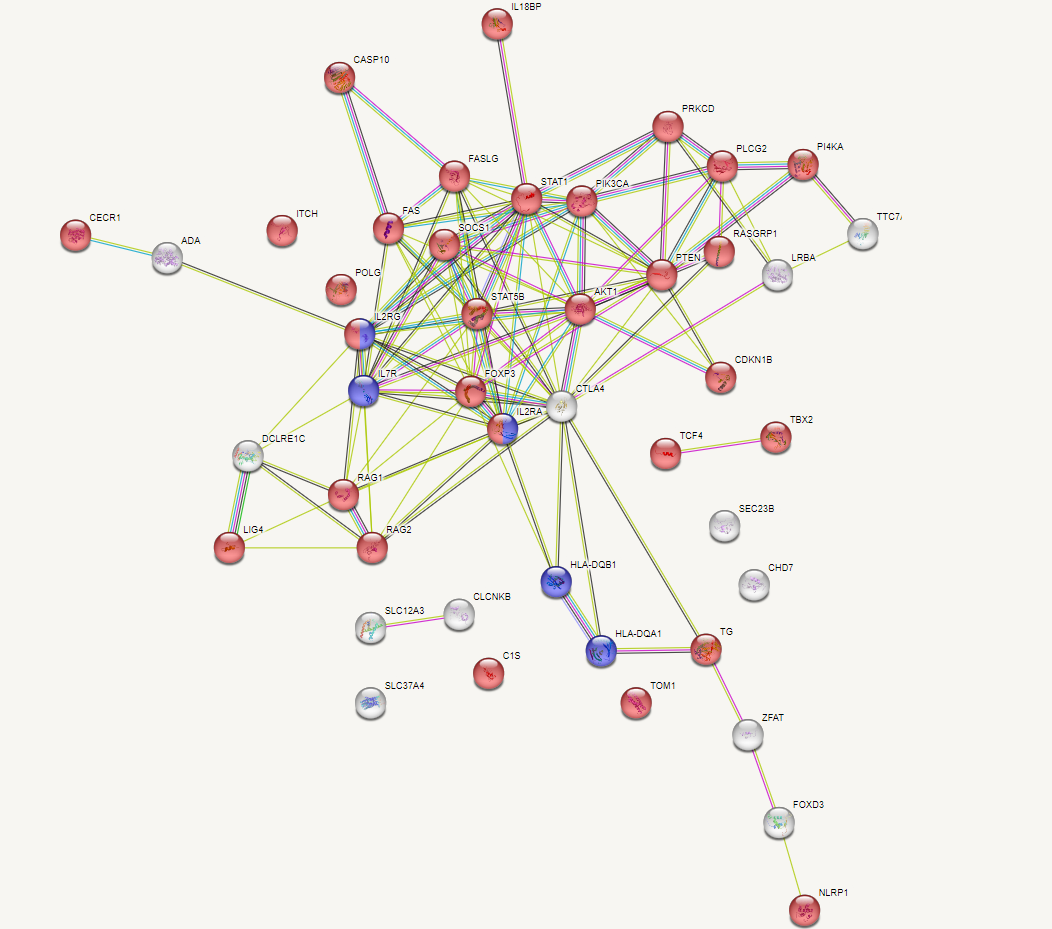
\includegraphics[scale=0.4]{figures/red de genes.png}
    
    Figure 2.1. Red de Genes
\end{center}
\\ \\
Dada la importancia de los factores genéticos en este fenotipo (HP:0100646), el estudio se centrará en la realización de un análisis de los diferentes genes asociados a dicho fenotipo y de las relaciones funcionales entre estos. 
\\ \\  \newpage 
Se tendrán en cuenta el tipo de interacción (física, co-expresión, databases, etc...) a partir de las cuales diluciar los diferentes clusters. Estos clusters ayudarán a clasificar genes en base a la función molecular que desempeñen. La distribución de genes resultante ayudará a descubrir cuales de ellos tienen una mayor relevancia.
\\ \\




